\documentclass[a4paper,12pt]{article}
%%%%%~~~~~~~~~~~~~~~~~~~~~usepackage~~~~~~~~~~~~~~~~~
\usepackage{rotating}
\usepackage[top=0.8in, bottom=0.8in, left=0.8in, right=0.8in]{geometry}
\usepackage{graphicx}
\usepackage[numbers,square,sort&compress]{natbib}
\usepackage{setspace}
\usepackage[cdot,mediumqspace,]{SIunits}
\usepackage{caption}
\usepackage{subcaption}
\usepackage{mathtools}
\usepackage{authblk} % to get affil
\usepackage{float} % to get figures where wanted
\usepackage{indentfirst} % to indent the first para of every chapter
\usepackage{listings}

%####################### new command

\newcommand{\myemail}{ayushi.singh@mail.utoronto.ca}
\newcommand{\anita}{anita.bahmanyar@mail.utoronto.ca}
\newcommand{\carly}{c.berard@mail.utoronot.ca}

%####################### Title and etc

\begin{document}
\onehalfspacing
\title{Astrometry from CCD Images}
\author{Ayushi Singh, Anita Bahmanyar, Carly Berard}
\affil{\small {\myemail}}%, {\anita}, {\carly}}
\affil{\small Astronomy and Physics, University of Toronto, ON}
\date{4 December, 2013}
\maketitle
%\altaffiltext{1}{{\myemail}}
%\altaffilmark{1}
%####################### Abstract

\begin{abstract}
\label{abstract}
This experiment examines the one dataset of NGC7331 galaxy and five dataset of 30 Urania asteroid. Python programming language and DS9 software was used to inspect, calculate and model the data. All the data was corrected for dark counts and flat-field. Using the centroids from NGC7331 data and USNO B-1.0 star catalog, plate constants were calculated that corrected for the CCD pixel to the celestial coordinate system. The plate constants were accurate with the error of 0.597 in $x_{pixels}$ and 0.476 in $y_{pixels}$. The $\chi^2$ for $x$ is 267.49, and for $y$ is 230.31. And, the $\chi_{red}^{2}$ for $x$ and $y$ is 1.45 and 1.24, respectively. Using these plate constants and the five datasets of 30 Urania asteroid, the proper motion of the asteroid was calculated, which is 35.496 $\pm$ 0.900 arcsec per hour. 
\end{abstract}

%####################### Introduction
\section{Introduction}
\label{sec:introduction}
The purpose of this experiment was to used the data collected from Dunlap Institute Telescope and detect the proper motion of the 30Urania Asteroid. Proper motion of object is change in angular position over some period of time. The object moving in space have velocity in two direction: radial velocity and transverse velocity. Proper motion is related to transverse velocity. In astronomy most of the objects are celestial; therefore, their proper motion is in the unit arc seconds over time. The time, however, varies depending on the objects. For stars, time is usually in terms of year. In this case, the candidate is an asteroid, which appears to moves faster relative to the stars. Hence, in this case time will be in seconds.
 \\
\indent The report explains the step by step process used to obtain the final result with errors. All the data provided were, firstly, corrected for the effect of CCD dark pixel and flat-field. Then, the data from USNO catalog, from the online link, with the data from a galaxy (NGC7331) was used to obtain the correction for CCD pixels to right ascension ($\alpha$) and declination ($\delta$). This correction gave plate constant values. Using these plate constants and the five dataset provided for asteroids  were used to calculate the proper motion of the asteroid in the sky, also with errors.

%####################### Equipment
\section{Equipment}
\label{sec:equipment}
The data was collected using Dunlap Institute Telescope (DIT) that was located at New Mexico Skies on Mt. Joy site near Mayhill, NM. It was a 50-cm robotic telescope dedicated to the search for optical counterparts of gamma-ray bursts. The telescope had 4096 $\times$ 4096 pixel CCD array, with the view of 36 $\times$ 36 arc minutes. The focal length being 3454 mm and with F/ratio = F/6.8 \cite{instructions}. Also, an online catalog was used to find correlation between CCD data and the location. It is called USNO B-1.0 star catalog that lists position and magnitude in various optical pass band. It was used to give us the position of the star below certain magnitude based on the CCD data coordinate.  For the data reduction, calculations and modeling, DS9 software and Python Programming Language was used. DS9 provided the visual representation of the data set, including all the statistic about the data in the header. And Python allowed to perform calculations and modeling of the data. 

%####################### Data
\section{Data Summary}
\label{sec:data}

The data was already collected before hand and the link to the data was provided to us at the start of this experiment on the course website \cite{instructions}. 


\begin{table}[H]
\centering % used for centering table
\caption{Summary of all the data collected for this experiment}
\tabcolsep 2.pt %\small
\footnotesize

\begin{tabular}{ccccccc}% centred columns (8 columns)
\hline
\hline
Data \# & Name & Date & Time & Right Ascension& Declination &Comments \\
& &  &[UTC time]&[hms J2000]&[dms +N J2000]&\\
\hline
\hline
1   &   NGC7331   &   13/10/2011  &03:18:59 &22 37 18.00&+34 26 37.0&map with galaxy\\
2   &   30 Urania    & 20/01/2012   &04:28:30&02 57 54.59&+19 14 41.9& Asteroid\\
3   &   30 Urania     &  21/01/2012   &04:40:27&02 58 49.61&+19 16 56.9&Asteroid \\
4   &    30 Urania   &23/01/2012    &05:43:40 &03 00 44.11&+19 21 45.0&Asteroid \\
5   &   30 Urania    & 24/01/2012    &04:26:48&03 01 43.55&+19 24 17.6& Asteroid\\
6   &  30 Urania  &  29/01/2012   &01:27:18 &03 07 01.64&+19 38 19.4&Asteroid \\
\hline
\hline

\end{tabular}
\label{table:dataset} % is used to refer this table in the text
\end{table}

Each dataset has 3 files provided in them. This includes, raw data, dark counts due to CCD and flat-field taken at either dawn or twilight. The flat-field has already been corrected. 
%####################### Data Reduction and Method
\section{Data Reduction and Method}
\label{sec:reduction}

\subsection{Correction for Dark and Flat-field}
\label{sec:dark}
The raw data of NGC7331 Galaxy, from Table \ref{table:dataset}, was a fits files. Using python module pyfits, the data from the files was extracted. It was in the form of 2-D image with 2048 $\times$ 2048 pixels. Initially the data is flipped in a way, that North is pointing down and East is pointing left. This is due the telescope, which records the inverted image. Therefore, the first step was to correct the image so that North is pointing up and East is pointing right. Then, to correct the data following equation was used:

\begin{equation}
\label{eq:flat}
\begin{array}{rcl}
    I_i &= \frac{R_i - D_i}{F_i} 
\end{array}
\end{equation}
Where $I_i$ is the corrected intensity value for the the pixel number $i$, which is calculated using the raw data ($R_i$), the dark counts ($D_i$) and the flats ($F_i$). However, Equation \ref{eq:flat} is not sufficient for the flat is not correct. The median of flat is $\sim$0.8, which should be 1. Therefore, the whole flat data set is divided by the median of the flat data set. This then gives us the corrected $F_i$.   

\subsection{Centroids of NGC7331 Galaxy}
\label{sec:centroid}
Using the corrected NGC7331 data was used to find the centroids of the prominent stars and galaxy. First, going though every pixels to find the one that are maximum of its surrounding and above a certain threshold intensity. If no threshold values is set, then every small peak will be included. Therefore, initially the background value be approximately 3631.9, which turn out to be too low. For there is no need for the very dim stars. Therefore, background threshold values was chosen to be 15000. This values is chosen because it provides the best match with the USNO catalog. \\
\indent There is overlapping and reoccurrence of maxima in the same star. To correct for the error. The following equations were applied on the maximum values. 

\begin{equation}
\label{eq:centroid}
\begin{array}{rcl}
   \vspace{0.3cm}
   \langle x \rangle &= {\sum_{i=1} x_i I_i}/ {\sum_{i=1} {I_i}}, \ \
   \langle y \rangle &= {\sum_{i=1} y_i I_i}/{\sum_{i=1} {I_i}} 
\end{array}
\end{equation}
Here ${\langle x \rangle}$ and ${\langle y \rangle}$ represent the value of $x$ and $y$ component of centroids, respectively. The box of $50 \times 50$ was created, with the centre being one the maximum value. Then all the pixel within the box, that has intensity value above 15000 (threshold intensity), were averaged using the Equation \ref{eq:centroid}. With $x_i$, $y_i$ and $I_i$ being the value of chosen pixel. 

\begin{figure}[H]
	\centering
	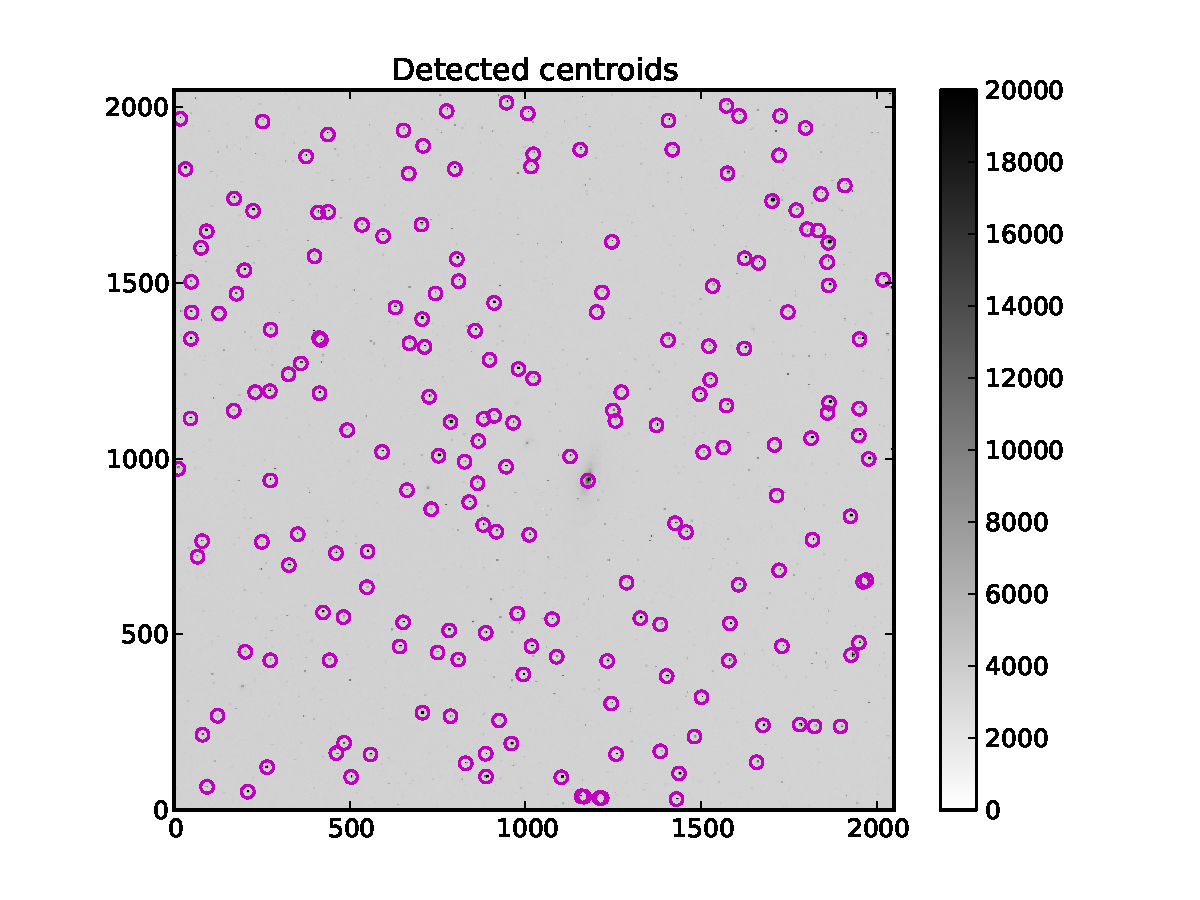
\includegraphics[angle=0,height=8cm,width=10.5cm]{galaxy/Centroids.pdf}
	\caption{Centroids of NGC7331 data that are above the threshold intensity of 15000 plotted in the negative color.}
	\label{fig:centroid}
\end{figure}

In the Figure \ref{fig:centroid}, the actual data is in negative colour. That is, the sky is grey where as the stars are black. The circles represent the centroids points around the stars, which has the intensity higher than the threshold value. 

\subsection{Matching Stars and Projected Coordinates}
\label{sec:matching}
Centroids of NGC7331 from Section \ref{sec:centroid} are match with the USNO B-1.0 star catalog \cite{usno}. First, using the centred $\alpha_0$ (22 37 18.00) and $\delta_0$ (+34 26 37.0) of NGC7331, from Table \ref{table:dataset}, data from the online catalog was extracted. This was done by changing the $\alpha_0$ and $\delta_0$ to radian by using the following conversion units for degree, hours, minutes and second. However, to manipulate the data it was changed into projected/standard coordinates using the following equations,

\begin{equation}
\label{eq:projected}
\begin{array}{rcl}
   \vspace{0.3cm}
   X &= -\frac{cos\delta sin(\alpha-\alpha_0)}{cos\delta_0 cos\delta cos(\alpha-\alpha_0)+sin\delta sin\delta_0}\\
   Y &= -\frac{sin\delta_0 cos\delta cos(\alpha-\alpha_0)-cos\delta_0 sin\delta}{cos\delta_0 cos\delta cos(\alpha-\alpha_0)+sin\delta sin\delta_0} 
\end{array}
\end{equation}

where, $\delta_0$ and $\alpha_0$ are the centre coordinate of the NGC7331 data converted into radian.  Here celestial sphere is taken to the unit radius. 

\begin{figure}[H]
	\centering
	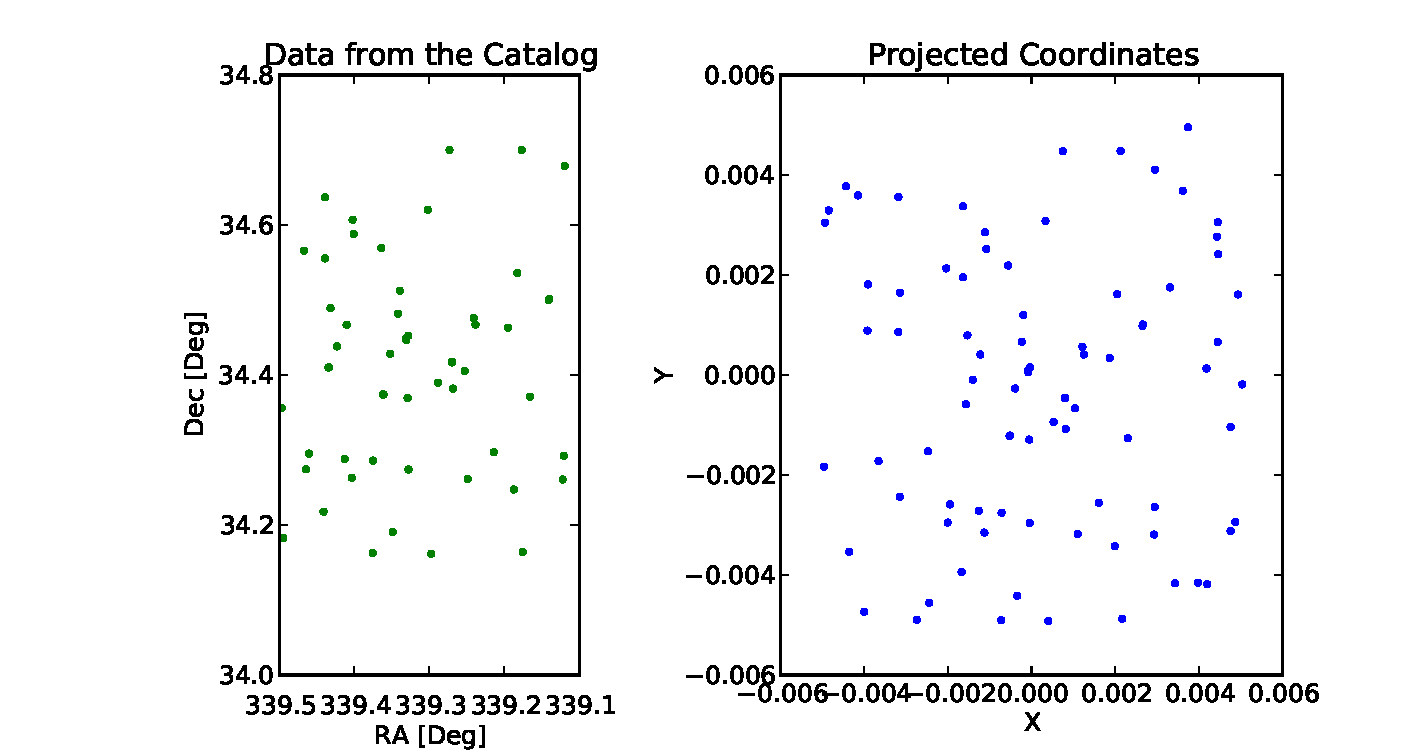
\includegraphics[angle=0,height=5cm,width=11cm]{galaxy/catalog.pdf}
	\caption{$\it{Left:}$ plot of USNO data in degrees using $\delta_0$ and $\alpha_0$ at the magnitude $>$ 0.13. $\it{Right:}$ plot of USNO data in projected coordinates.}
	\label{fig:catalog}
\end{figure}

In Figure \ref{fig:catalog}, the data from catalog is represented in two coordinate system. The degree based plot is narrowed rectangle but the transformation to projected coordinate transformed it into a square image. There are very few stars because the magnitude $>$ 0.13. Using these coordinated, cataloged was transformed to pixel coordinates by following equations,

\begin{equation}
\label{eq:pixel}
\begin{array}{rcl}
   \vspace{0.3cm}
   x &= f(X/p)+x_0\\
   y &= f(Y/p)+y_0
\end{array}
\end{equation}

where $x$ and $y$ are the transformed pixel value. $f$  (focal length of telescope) is 3454 mm, from Section \ref{sec:equipment}. $p$ (pixel size) is 0.0018 mm, $x_0$ = $y_0$ = 1024 \cite{instructions}. This is an ideal case that works for the perfect CCD camera. 

%####################### Calculation and Modeling
\section{Calculation and Modeling}
\label{sec:calc}

\subsection{Plate Constants}
\label{sec:plate}

With centroids in pixels and USNO data converted into pixels using Equation \ref{eq:projected} and \ref{eq:pixel}, the two data can be compared. 

\begin{figure}[H]
	\centering
	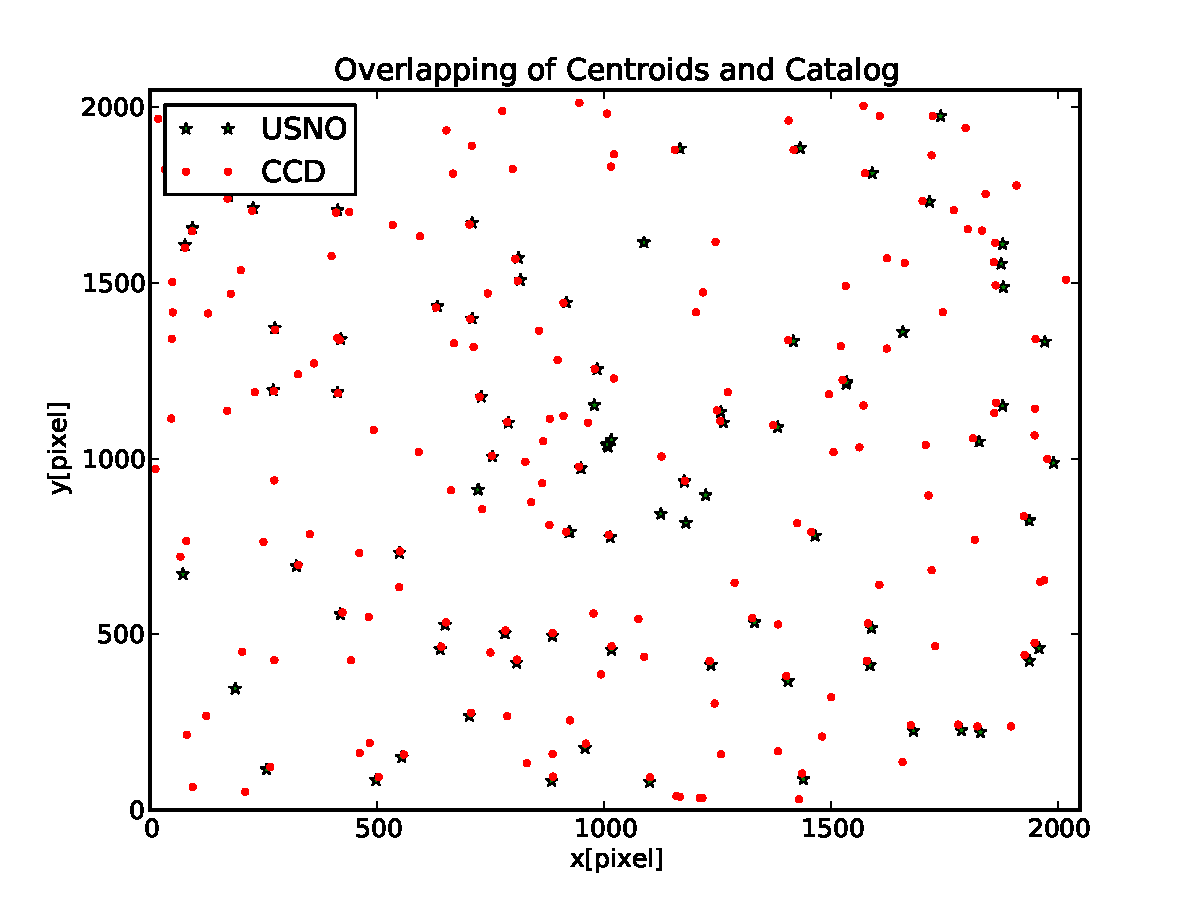
\includegraphics[angle=0,height=7cm,width=8cm]{galaxy/Overlapping.pdf}
	\caption{Plots of CCD centroids and the data for the USNO catalog}
	\label{fig:match}
\end{figure} 
In the Figure \ref{fig:match}, the two data is over plotted. It is clear that there are some matches, however there are some stars in catalog that have no centroid match and come centroid that have no catalog match. For the further calculation only centroids and catalog points that are matched are used.  

\begin{figure}[H]
	\centering
	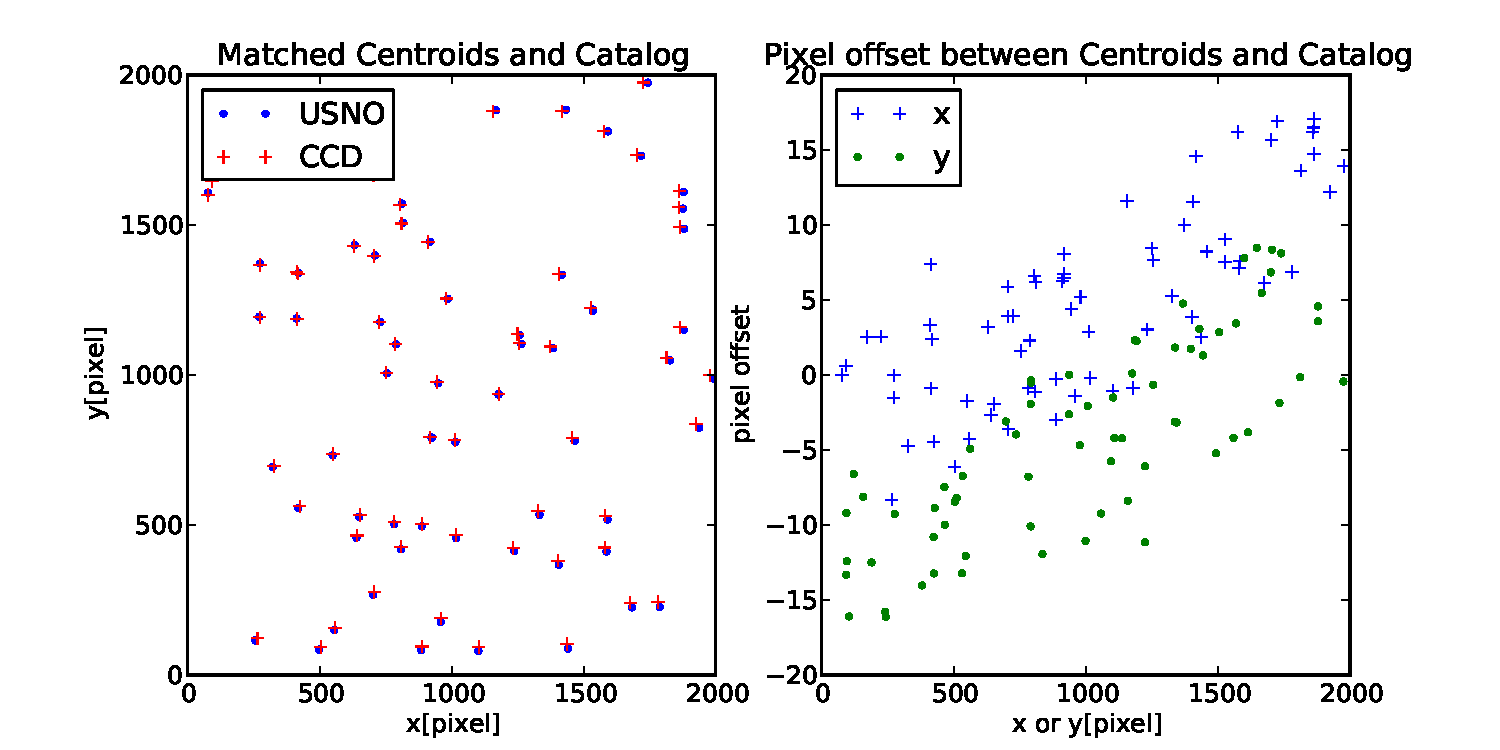
\includegraphics[angle=0,height=5cm,width=11cm]{galaxy/offset.pdf}
	\caption{$\it{Left:}$ plot of only the centroids and catalog points that are matched with each other. $\it{Right:}$ offset plot of residuals between centroids and catalog data in x and y coordinates.}
	\label{fig:offset}
\end{figure}
In the Figure \ref{fig:offset}, the residual have a linear trend and are spread in wide range. To correct for this, better equation is required to replace Equation \ref{eq:pixel} and calculate plate constant. \\

\begin{equation}
\label{eq:newpixel}
	\bf{x}= \bf{TX}
\end{equation}

where $\bf{X}$ = ($X,Y,1$), $\bf{x}$ = ($x,y,1$) and 

\begin{equation}
\label{eq:T}
\begin{array}{rcl}
\bf{T}&= \begin{bmatrix}
      			(f/p)a_{11}&(f/p)a_{12}& x_0\\
      			(f/p)a_{21}&(f/p)a_{22}& y_0\\
      			0& 0 & 1
		\end{bmatrix}
\end{array}
\end{equation}
Equation \ref{eq:newpixel} is the new equation for not ideal CCD camera that replaces Equation \ref{eq:pixel}. From Equation \ref{eq:T}, the six plate constants are introduces are 4 $a_{ij}$ values, $x_0$ and $y_0$. These are calculated using following equation:

\begin{equation}
\label{eq:values}
\begin{array}{rcl}
\bf{a}&= \begin{bmatrix}
      			x_1\\
			\vdots\\
      			x_N
		\end{bmatrix},
\bf{B}&= \begin{bmatrix}
      			(f/p)X_{1}&(f/p)Y_{1}& 1\\
			\vdots&\vdots&\vdots\\
      			(f/p)Y_{N}&(f/p)Y_{N}& 1
		\end{bmatrix}, 
\end{array}
\end{equation}
 
\begin{equation}
\label{eq:c}
	\bf{c}= \bf{(a-Bc)^{T}B^{T}a}
\end{equation}
where $\bf{c}$ = $(a_{11},a_{12}, x_0)$, similar method can be used to calculate  $\bf{d}$ = $(a_{21},a_{22}, y_0)$. As a result the plate constants we get are: 

\begin{equation}
\label{eq:cd}
\begin{array}{rcl}
\bf{c}&= \begin{bmatrix}
      			0.991, \ \
			0.00669, \ \
      			1019.14
		\end{bmatrix}, \ \
\bf{d}&= \begin{bmatrix}
      			0.00667, \ \
			0.990, \ \
      			1027.90
		\end{bmatrix}
\end{array}
\end{equation}
Then using Equation \ref{eq:newpixel} and \ref{eq:T}, corrected pixel value for $x$ and $y$. 

\begin{figure}[H]
\centering
$\begin{array}{cc}
	\hspace{-1.5cm}
	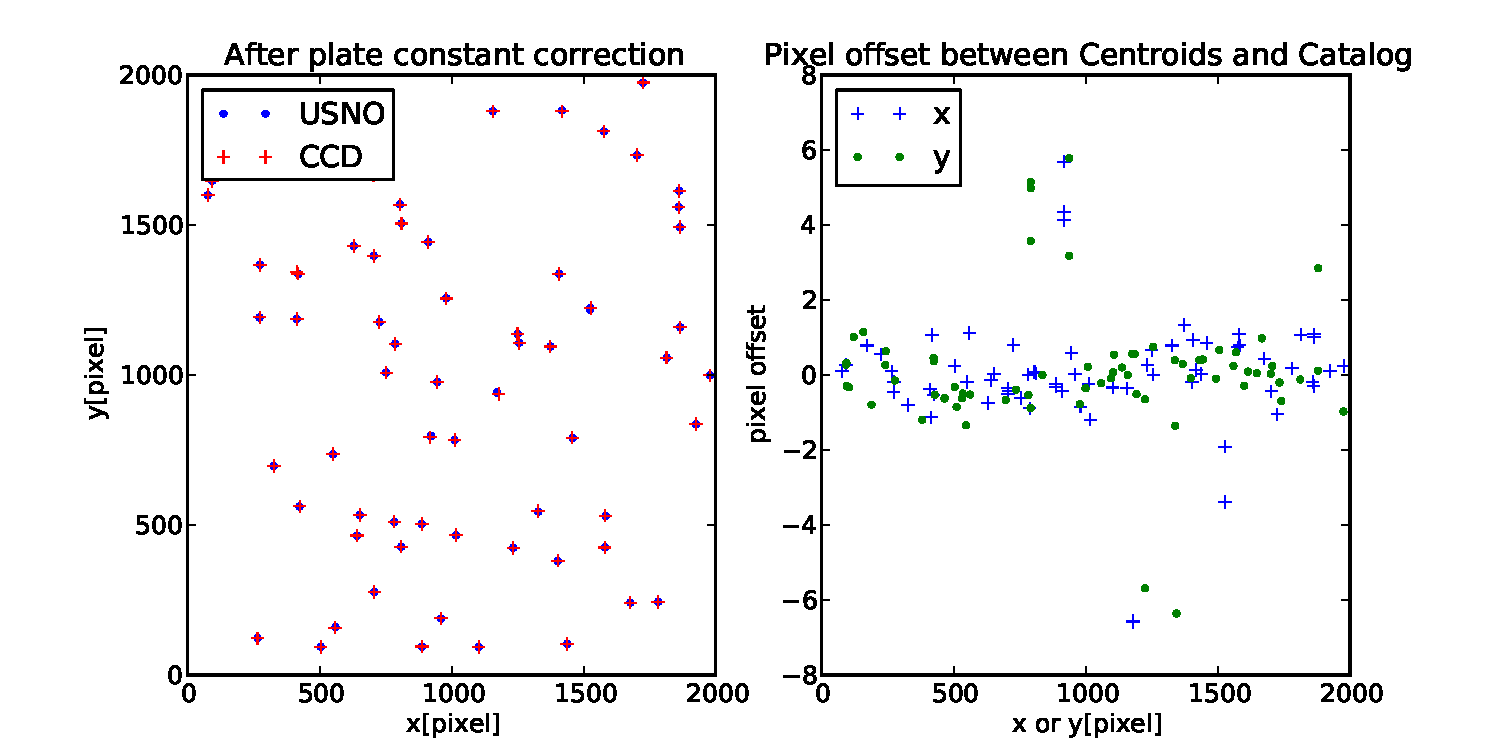
\includegraphics [angle=0,height=6cm,width=14cm]{galaxy/offsetnew.pdf} &
	\hspace{-1.5cm}
	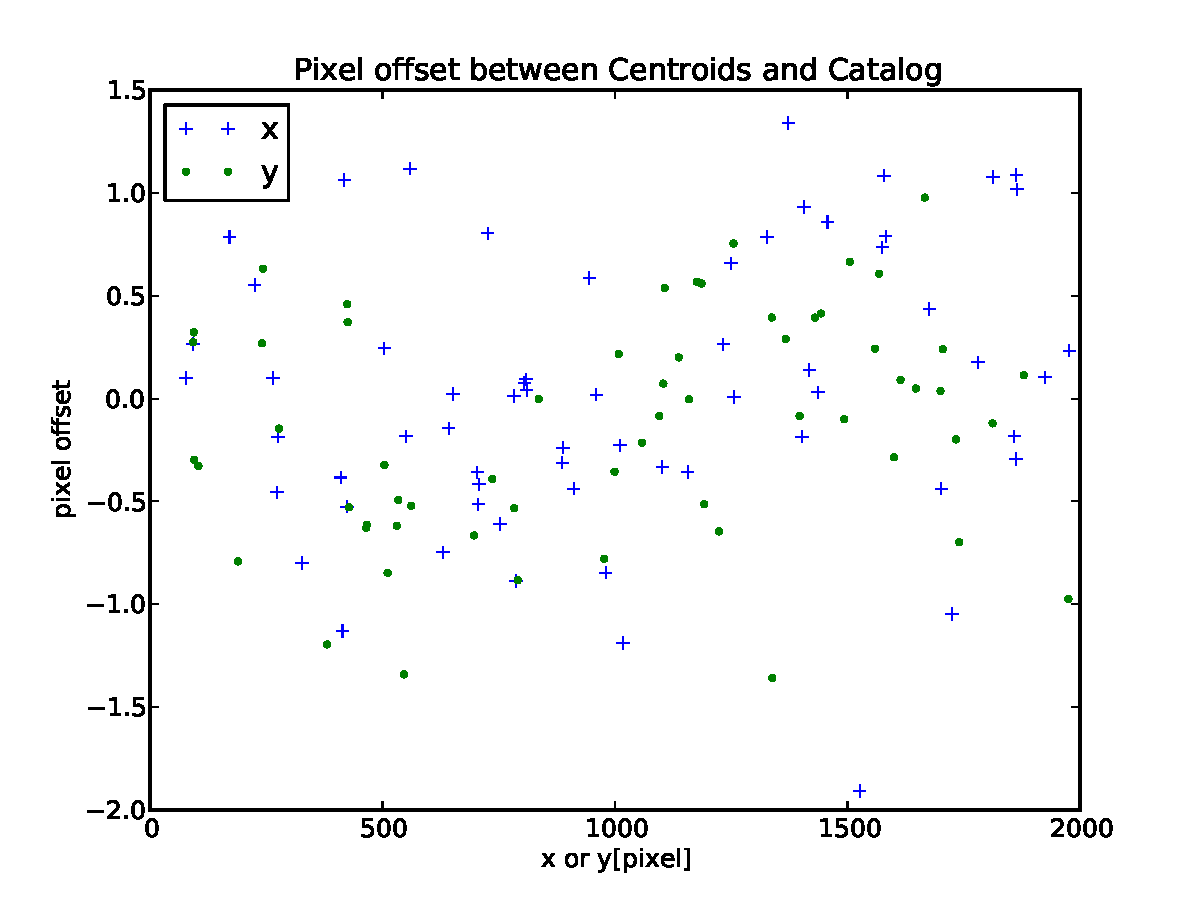
\includegraphics[angle=0,height=5cm,width=7cm]{galaxy/offsetcorrected.pdf} \\
\end{array}$
\caption{$\it{Left:}$ plot of only the centroids and catalog points that are matched with each other. $\it{Middle:}$ offset plot of residuals without the poor match. $\it{Right:}$ offset plot of residuals without the poor match.}
\label{fig:newoffset}
\end{figure}

Compared Figure \ref{fig:offset}, Figure \ref{fig:newoffset} provides much better residual. In the $\it{Left}$ side, the centroids and the catalog has a very good match, $\it{Middle}$ one shows the good residuals within the range of -2 to 2 pixels. The outsider are the one that are not a good match, and therefore not a star. Disregarding those  $\it{Right}$ side is obtained and used to calculate errors. 

\begin{equation}
\label{eq:SD}
\begin{array}{rcl}
	\vspace{0.3cm}
	\mu &= \frac{\sum x_i}{N}, \ \
	\sigma &= \sqrt{\frac{\sum x_i - \mu}{N-1}}
\end{array}
\end{equation}
where $\mu$ is the mean and $N$ is number of samples, $\sigma$ is the standard deviation. This gave the error in $x$ and similarly, it was used to obtain error in $y$, which is 0.597 in $x$ and 0.476 in $y$. 

\subsection{Proper motion of Asteroid 30 Urania}
\label{sec:proper}
Now working with the dataset 2-6 from Table \ref{table:dataset}. First the data is corrected for flats and dark as explained in Section \ref{sec:dark}. Then, using the centroids method from Section \ref{sec:centroid} with the threshold intensity of 5000, stars of all 5 dataset are recorded. In Section \ref{sec:plate}, the method is explain to get from celestial coordinates to pixel. However, using the same plate constant as in Equation \ref{eq:cd} and the inverse formula of Equation \ref{eq:newpixel}, solution from pixel to projected coordinate can be obtained. Then using following equations, they are converted from projected coordinate to celestial coordinates.

\begin{equation}
\label{eq:angle}
\begin{array}{rcl}
   \vspace{0.3cm}
   tan(\alpha-\alpha_0) &= -\frac{X}{cos\delta_0 -Ysin\delta_0}\\
   sin(\delta) &= \frac{sin\delta_0+Ycos\delta_0}{(1+X^2+y^2)^{1/2}} 
\end{array}
\end{equation}

\begin{figure}[H]
	\centering
	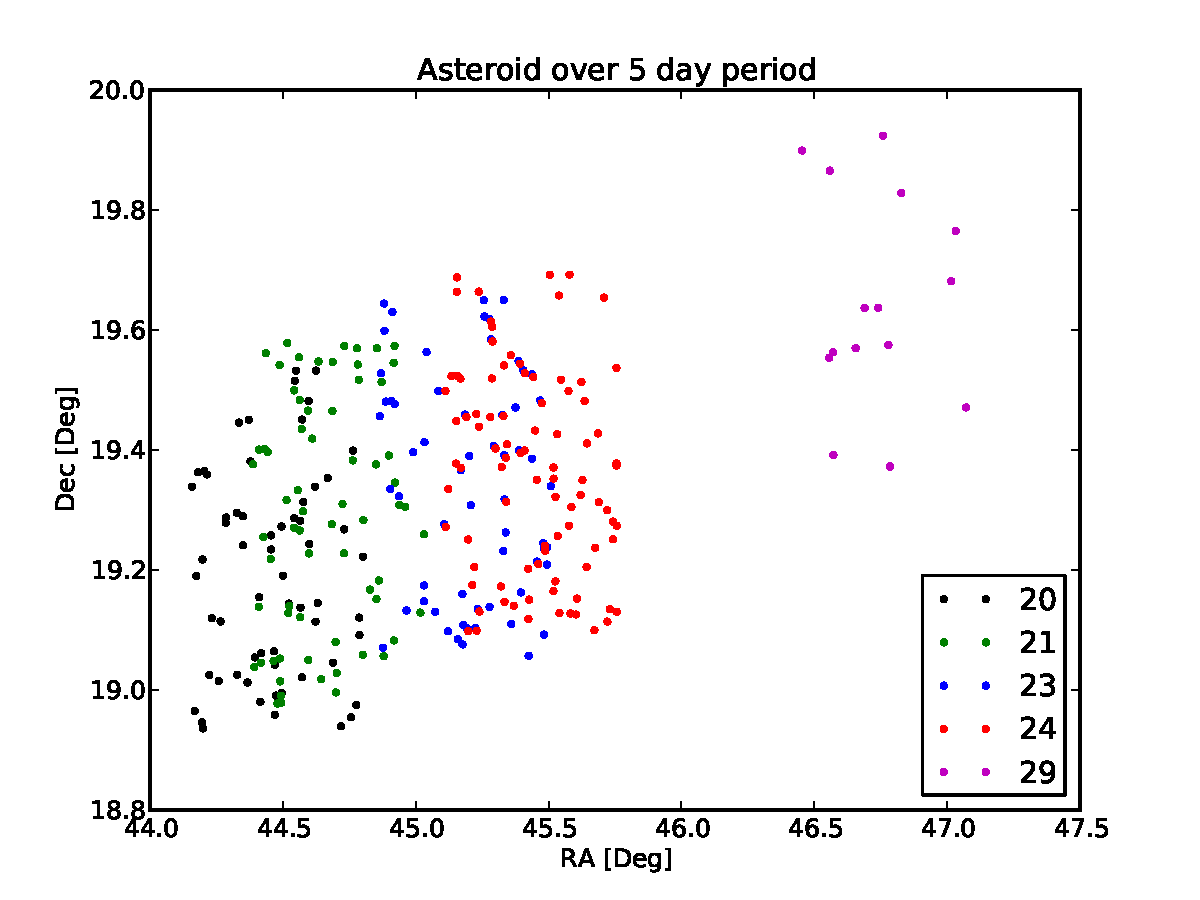
\includegraphics[angle=0,height=8cm,width=11cm]{asteroid/Chartfull.pdf}
	\caption{Data from five days converted into degree.}
	\label{fig:chart}
\end{figure}
Here the data five, taken on $28^{th}$, is ignored in later later calculation because it's way off. And from the rest of the data, it is clear that there is a correlation, however it's will not help in finding asteroid. Therefore, using DS9, asteroids in the first 4 dataset was taken out to be:

\begin{table}[H]
\centering % used for centering table
\caption{$x$ and $y$ pixels of asteroid}
\tabcolsep 2.pt %\small
\footnotesize

\begin{tabular}{ccccccc}% centred columns (8 columns)
\hline
\hline
Date & $x_{pixels}$ & $y_{pixels}$  \\
\hline
\hline
20   &   1086 & 992\\
21   &    1089& 1007\\
23   &    1063 & 1039\\
24   &  1087&1008\\
\hline
\hline

\end{tabular}
\label{table:pixel} % is used to refer this table in the text
\end{table}
Using these pixels values, asteroid was plotted.

\begin{figure}[H]
\centering
$\begin{array}{cc}
	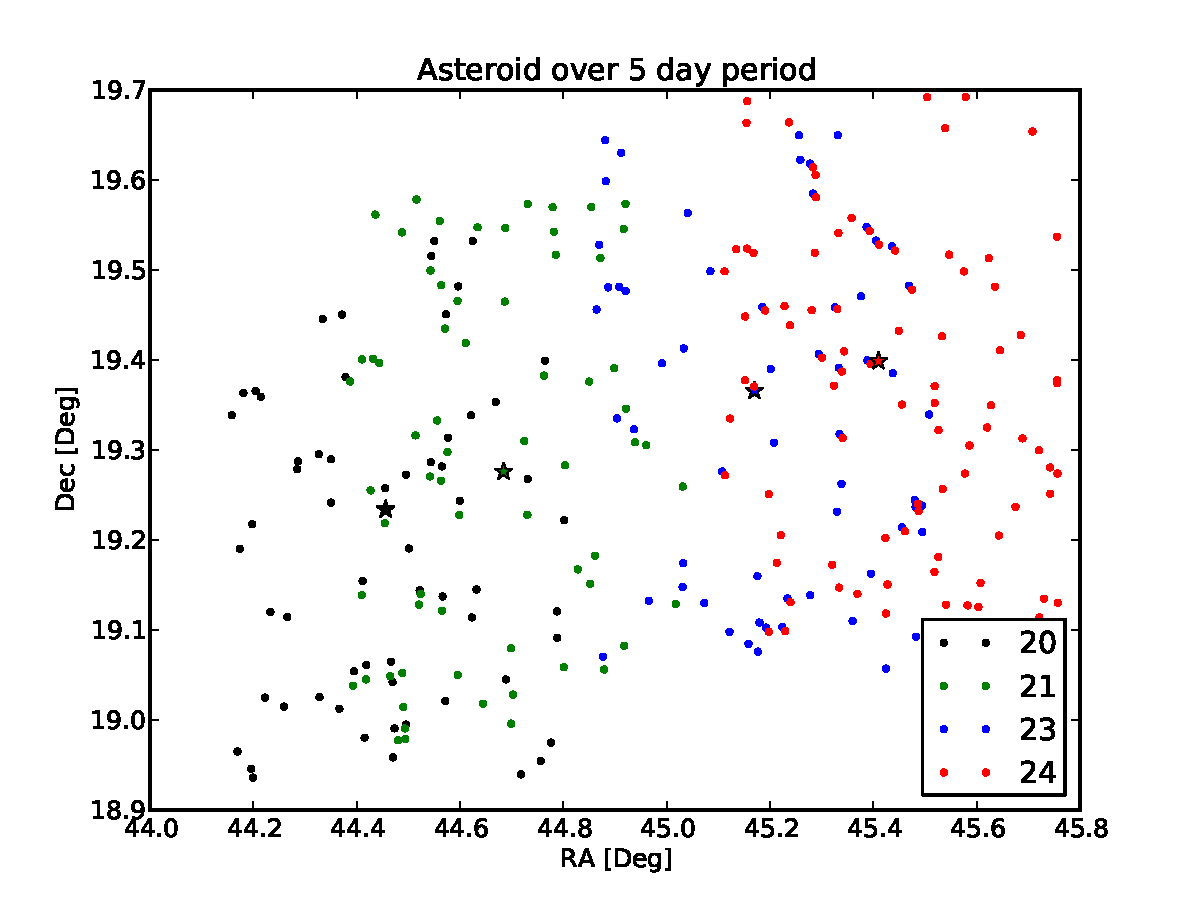
\includegraphics [angle=0,height=6cm,width=7cm]{asteroid/Chart.pdf} &
	\hspace{-0.2cm}
	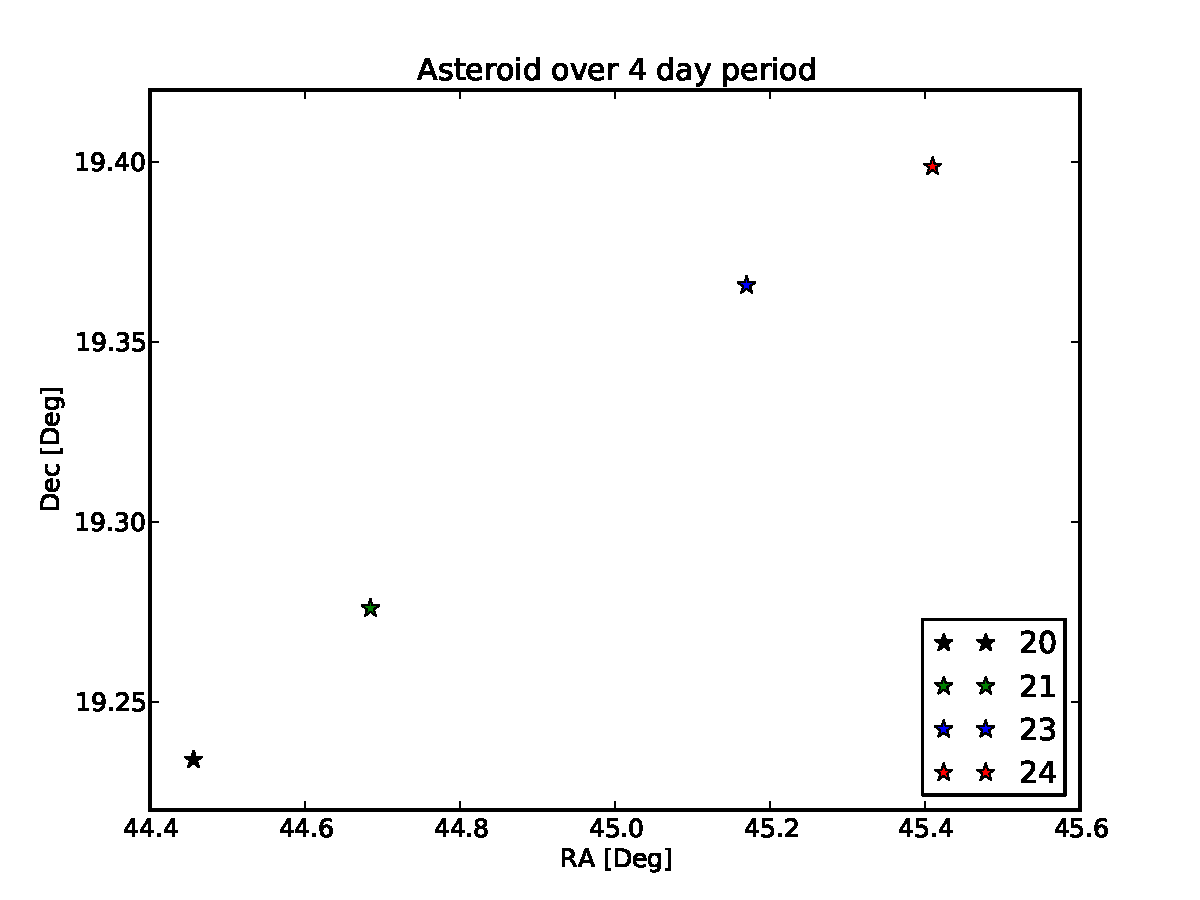
\includegraphics[angle=0,height=5cm,width=7cm]{asteroid/Asteroid.pdf} \\
\end{array}$
\caption{$\it{Left:}$ Data of first four days with the asteroid $\it{Right:}$ position of  the asteroid in four dataset}
\label{fig:newoffset}
\end{figure}
First image of Figure \ref{fig:newoffset}, only show the data from the first 4 night and the asteroid is clearly identify by a data point. From that we get the second image that has only asteroid, as qualitatively the asteroid did show a linear pattern. 

\begin{table}[H]
\centering % used for centering table
\caption{Time difference calculated with respect to the first night}
\tabcolsep 2.pt %\small
\footnotesize

\begin{tabular}{ccccccc}% centred columns (8 columns)
\hline
\hline
Data \# & Name & Date & Time from 00:00:00 &Time difference  \\
& & [01/2012] &[s]&[s]&\\
\hline
\hline
1   &   30 Urania   &  20   &16,110& 0\\
2   &   30 Urania   &  21   &16,827&87,117 \\
3   &   30 Urania   &  23     &20,620&263,710 \\
4   &   30 Urania   &  24    &16,008& 345,498\\
%5   &  30 Urania    &  29   &5,238& 766,728\\
\hline
\hline

\end{tabular}
\label{table:time} % is used to refer this table in the text
\end{table}

This table give the time difference between the first night and the subsequent nights in seconds. It is required to calculate the proper motion of the star. 
% for 2  16,827 +86400 - 16110 = 87117
\begin{equation}
\label{eq:proper}
\begin{array}{rcl}
   \vspace{0.3cm}
   distance &= \sqrt{(x_2-x_1)^2 + (y_2-y_1)^2}\\
\end{array}
\end{equation}
Then the proper motion is distance/time, where time is from Table \ref{table:time}. This gave the answer in degree/sec. Therefore, it is multiplied by 3600 to get the answer in arcsec per sec. So, the result is:
\begin{table}[H]
\centering % used for centering table
\caption{Proper motion solution between two night}
\tabcolsep 2.pt %\small
\footnotesize

\begin{tabular}{ccccccc}% centred columns (8 columns)
\hline
\hline
Date & Proper Motion (arcsec/sec) \\
\hline
\hline
20 - 21  & 0.00959  \\
20 - 23  &  0.00991 \\
20 - 24  &  0.01008  \\
\hline
\hline

\end{tabular}
\label{table:proper} % is used to refer this table in the text
\end{table}

Here we see a increasing tread over night. However they are still quite close. Therefore, the proper motion value can be averaged value, which is 0.00986 $\pm$ 0.00025 arcsec per sec, which is 35.496 $\pm$ 0.900 arcsec per hour, using Equation \ref{eq:SD}.
%###########################################################################################################################################################################

%####################### Discussion 
\section{Discussion}
\label{sec:discuss}
\subsection{NGC7331 Galaxy and the plate constants} 
\label{sec:galaxy}

It is essential to for correct any data used for errors. In this case, those two errors were dark and flat-field. Dark counts give hot pixels. It is taken with closed telescope so no light is passing though to get the effect of hot pixels. Therefore it's the value that is subtracted from the raw data as in Equation \ref{eq:flat}. Flat-field is the telescopic effect that is calculated at the time of dawn or twilight, which is divided from the raw data. In this case, both dark and flat were provided with the raw data for each dataset.
\begin{figure}[H]
\centering
	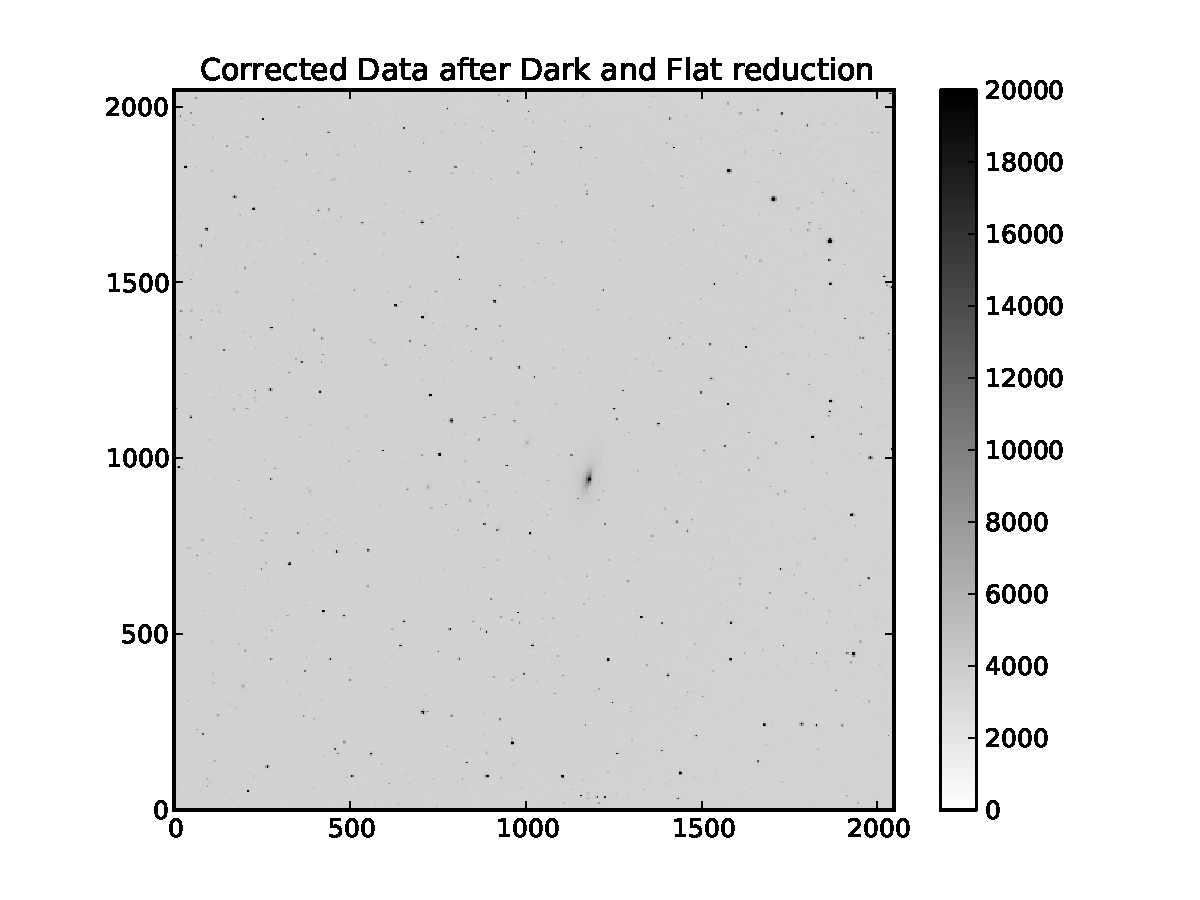
\includegraphics [angle=0,height=7cm,width=9cm]{galaxy/Corrected2.pdf} 
\caption{Corrected image of NGC7331}
\label{fig:correct}
\end{figure}
FIgure \ref{fig:correct} is the the proper image after correcting for dark and flat-field. It is also noted that all the images are inverted right-side up, to get the proper orientation of the data, with North up and East right. This is necessary because pixel to celestial coordinate requires them to be in right orientaiton. \\

\indent In Section \ref{sec:matching} and \ref{sec:plate}, the method of deriving plate constants is explained. But to consider it's effect, the two result from Figure \ref{fig:offset} and \ref{fig:newoffset}, needs to be compared. For the first one, only the ideal condition were assumed, which in this case where not correct. When plotting the image we see that there is rotation between centroids and the USNO data. Therefore, plate constants are used that correct for the rotation, shear, and scaling and the offset in the pixel. There after the correction using plate constants from Equation \ref{eq:cd}, in Figure \ref{fig:newoffset}, the result is much better with the residual between -2 and 2. To analyze the errors in plate constants, $\chi^2$ and $\chi_{red}^2$ values are calculated using the following equations.

\begin{equation}
\label{eq:chi}
\begin{array}{rcl}
   \vspace{0.3cm}
   \chi^2 &= \bf{(a-Bc)^{T} (a-Bc)}\\
   \chi_{red}^2 &= \chi^2/dof
\end{array}
\end{equation}

With very little errors $\chi^2$ and $\chi_{red}^2$ values are equal to 1. $\chi_{red}^2$ = 1 represents the best possible solution with very little to no errors. From the NGC7331 and USNO data the $\chi^2$ values are  267.49 for $x_{pixel}$, and 230.31 for $y_{pixel}$ . And, the $\chi_{red}^{2}$ values are  1.45 for $x_{pixel}$, and 1.24 for $y_{pixel}$. Despite the high $\chi^2$ value, $\chi_{red}^2$ is quite reasonable with values close to one. However, they are bit high than one, implying that errors are bit underestimated. \\

\indent The information about equipment from Section \ref{sec:equipment} states $f$ = 3454 mm and $p$ = 0.018 mm. Therefore $f/p \approx 192000$ pixel/radian. However, this value can be calculated using the plate constants by following equation. 

\begin{equation}
\label{eq:det}
\begin{array}{rcl}
   \vspace{0.3cm}
   f/p &= \sqrt{det(\bf{T})}
\end{array}
\end{equation}

By computing this, $f/p \approx 190061$ pixel/radian, which in quite close to the theoretical number 192000. This shows that the plate constants calculated are off by big value.

\subsection{30 Urania and Proper Motion} 
\label{sec:asteroid}

In Section \ref{sec:proper}, using the dataset 2-5 from Table \ref{table:dataset}, proper motion of the asteroid 30 Urania was calculated to be 35.496 $\pm$ 0.900 arcsec per hour from Table \ref{table:proper}. In this only the first for data were used because the last one was quite off and it was difficult to identify the position of the asteroid in the last dataset. However, it is necessary to verify if the data collected had correct co-ordinates and there was no systematic errors from the telescope. To achieve this, the position of the asteroid was recorded using DS9 and was match with the online library called JPL catalog \cite{jpl}.  

\begin{table}[H]
\centering % used for centering table
\caption{Comparing coordinates of asteroid from Telescope to JPL}
\tabcolsep 2.pt %\small
\footnotesize
\begin{tabular}{ccccc}% centred columns (8 columns)
\hline
\hline
Date & Telescope $\alpha$ &Telescope $\delta$&JPL $\alpha$ JPL$\delta$\\
\hline
\hline
20  & 2 57 49.05 & +19 14 29.5 &02 57 49.18 &+19 14 30.6  \\
21   &  2 25 44.36 & +19 16 46.6&02 58 44.50 & +19 16 46.1\\
23  &  3 00 41.10 & +19 21 38.9  &03 00 41.28& +19 21 39.5\\
24 & 3 01 37.18 & +19 24 03.6&03 01 37.42& +19 24 03.6\\
\hline
\hline

\end{tabular}
\label{table:match} % is used to refer this table in the text
\end{table}

It is clear that these values are same. Therefore, data collected from telescope is at correct position. Then, the proper motion of 35.496 $\pm$ 0.900 arcsec per hour is the correct result for the Asteroid 30 Urania.
\bibliographystyle{plain}
\bibliography{references.bib}
\end{document}
